%------------------------------------------------------------------------------
\chapter[Introdução]{Introdução}
\label{chap:introduction}
%------------------------------------------------------------------------------

Exemplo de uma citação \cite{HennessyPatterson2012}. Exemplo de referência de
figura: conforme pode ser observado na Figura \ref{fig:biblioteca}.

\lipsum [5 - 10]

\begin{figure}[t]
  \caption{Imagens de uma biblioteca.}
  \begin{subfigure}{.5\linewidth}
    \centering
    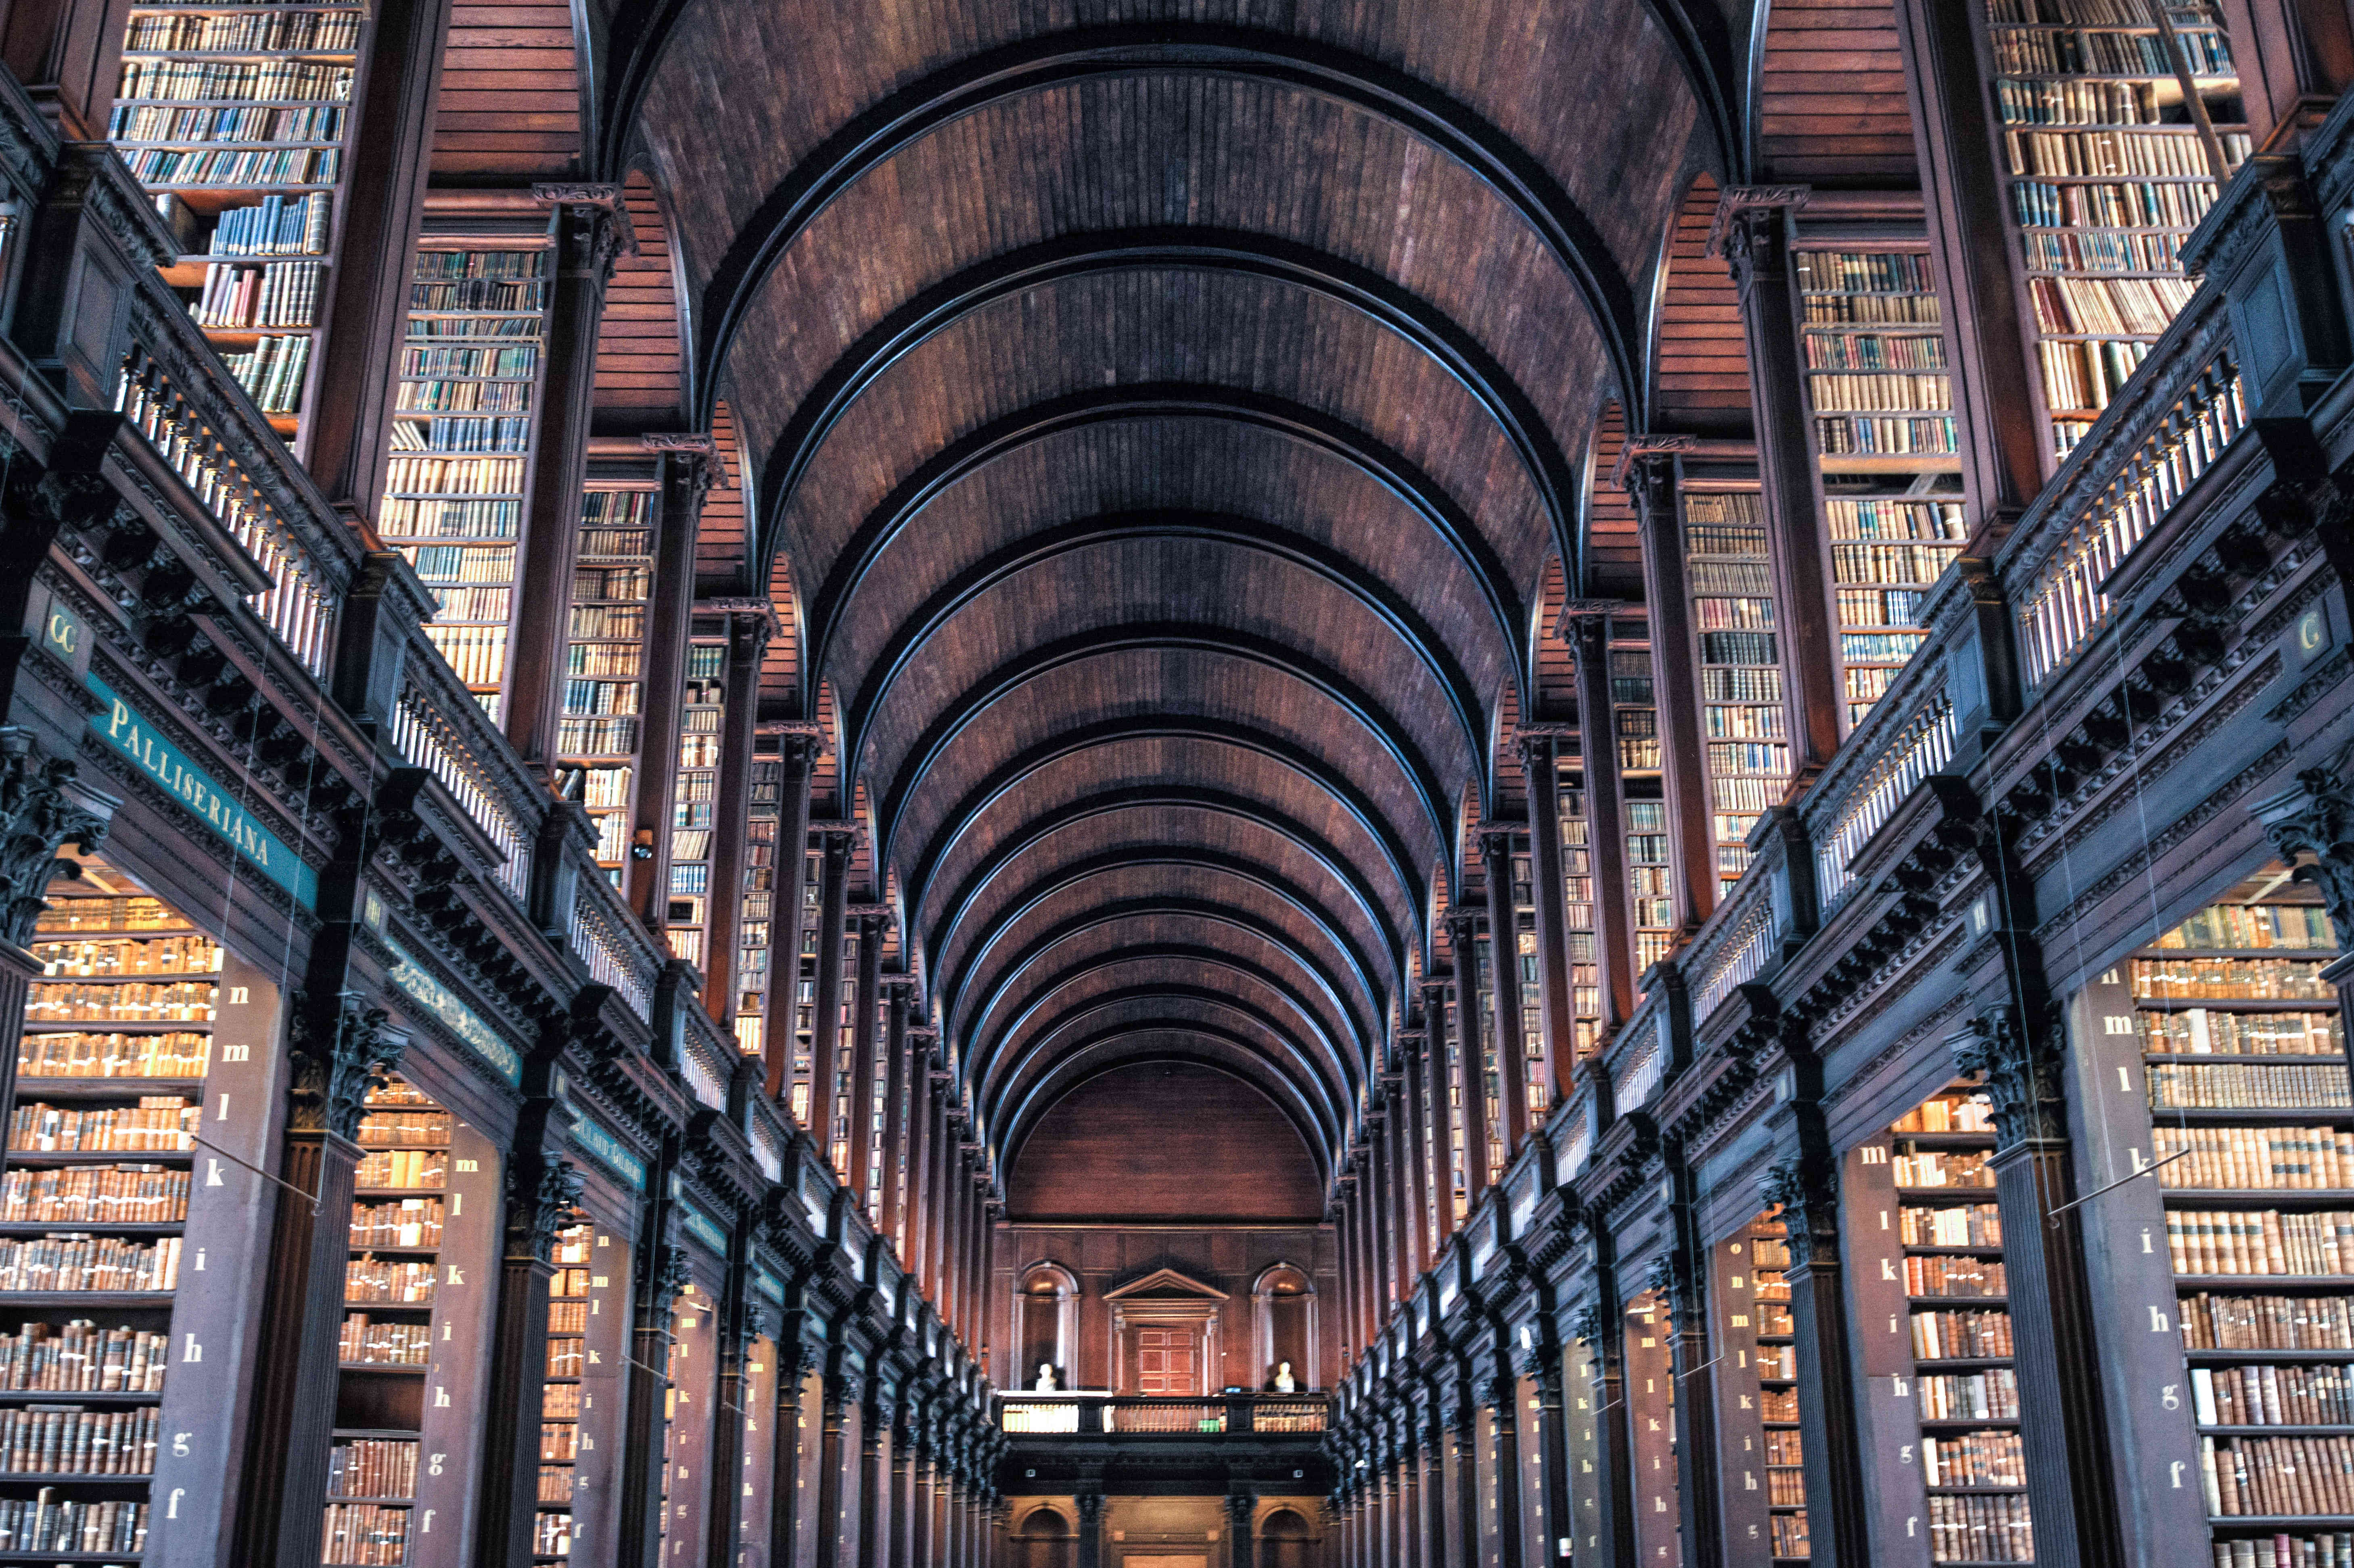
\includegraphics[width=\textwidth]{images/library1.jpg}
    \caption{Foto 1}
    \label{fig:foto1}
  \end{subfigure}
  \begin{subfigure}{.5\linewidth}
    \centering
    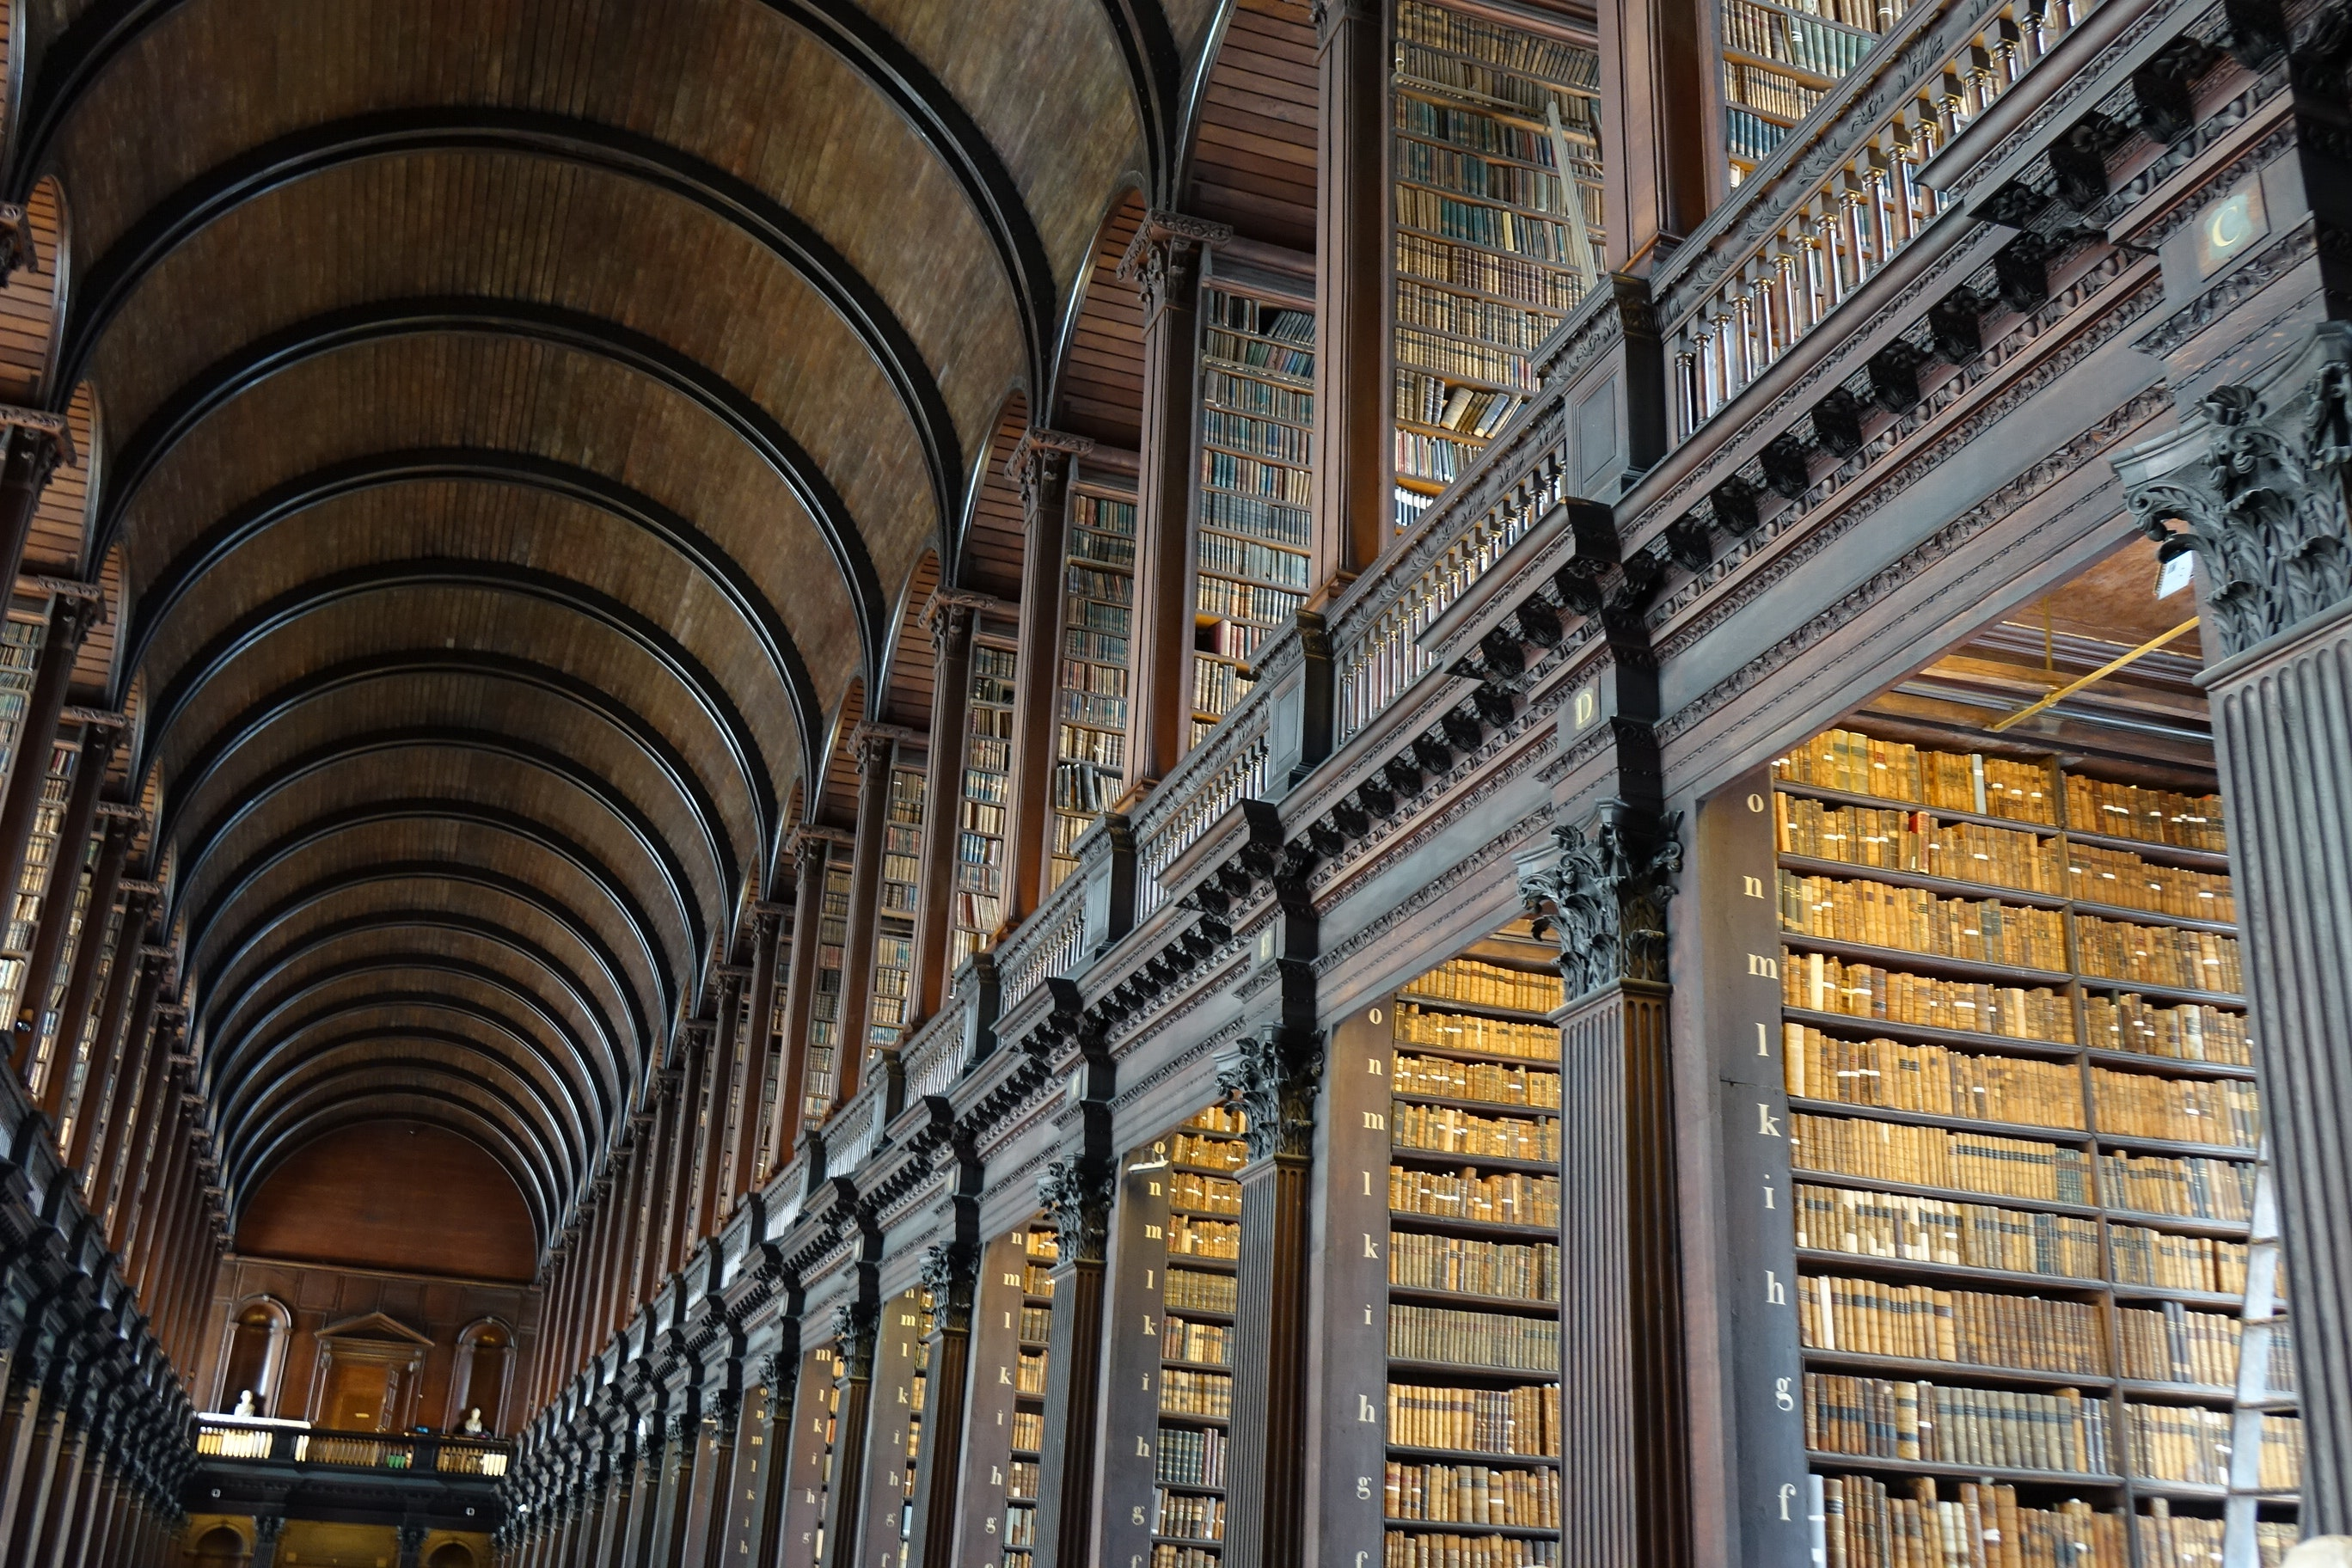
\includegraphics[width=\textwidth]{images/library2.jpg}
    \caption{Foto 2}
    \label{fig:foto2}
  \end{subfigure}
	\fonte{Extraído de ...}
  \label{fig:biblioteca}
\end{figure}


%------------------------------------------------------------------------------
\section{Objetivos e Contribuições}
\label{sec:objetivos}
%------------------------------------------------------------------------------

\lipsum[1 - 2]

%------------------------------------------------------------------------------
\section{Organização do Texto}
\label{sec:organizacao}
%------------------------------------------------------------------------------

\lipsum[3 - 3]
